Orodja na avtomatih so največkrat narejena iz HSS, 
hitroreznega jekla. To so jekla z dodanim kromom, volframom, 
molibdenijem, vanadijem in kobaltom. Na splošno, skupna količina 
legirnih elementov ne presega 7\%. Trdnost teh jekel je zelo visoka, 
od 63 do 67 HRC.

Uporabljajo pa se prav zaradi te visoke trdnosti. Z uporabo 
brusilnega stroja ali brusilke, se surovec obdela v nož po želji. 
Iz njih lahko naredimo katerokoli orodje; stružne, odrezne, 
profilne nože, kot tudi topovske svedre in pestiče. Surovci so 
največkrat dolgi 200 mm in kvadratni z standardnimi merami 
(8x8, 10x10, 12x12, 16x16…). Nekaj primerov navadnih surovcov
je na spodnji sliki \ref{hss_nozi}.

\begin{figure}[H]
    \begin{center}
        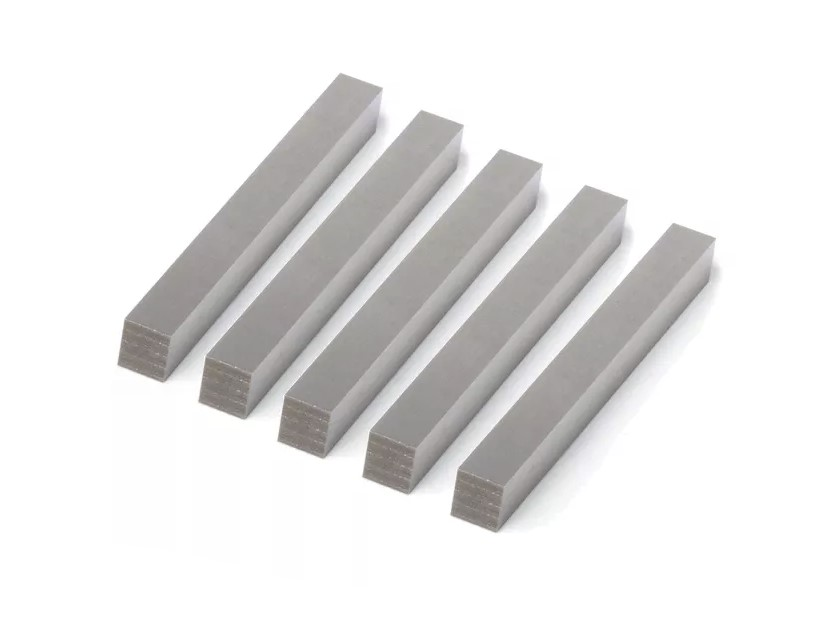
\includegraphics[width=\linewidth]{hss_nozi.jpg}
        \caption{HSS surovci
        \cite{hss_nozi}}
        \label{hss_nozi}
    \end{center}
\end{figure}

Obstojnost hitroreznih jekel v primerjavi z ostalimi ni najboljša, 
lahko se pa izboljša z raznimi prevlekami. Zaradi tega, se za 
avtomatna jekla uporablja večinoma HSS, za trša jekla, nerjavna 
in poboljšana, se pa uporabljajo noži iz karbidnih trdnin ali 
WIDIA. Narejeni so z postopkom sintranja in nam omogočajo veliko 
večje rezalne hitrosti in obrate pri mali obrabi.

\newpage
\subsubsection{Rezalna hitrost}
Rezalna hitrost je odvisna od materiala, ki ga obdelujemo, 
obdelovalnega postopka, prereza odrezka, hitrosti podajanja 
in željene površine (groba ali fina). Vrednosti rezalne hitrosti 
najdemo v tabelah, ki so bile narejene na podlagi preizkušanja 
in je nikoli ne računamo. Spodaj na sliki \ref{rezalna_hitrost}
je primer tabele rezalnih hitrosti vzetih iz Krautovega strojniškega
priročnika.

\begin{figure}[H]
    \begin{center}
        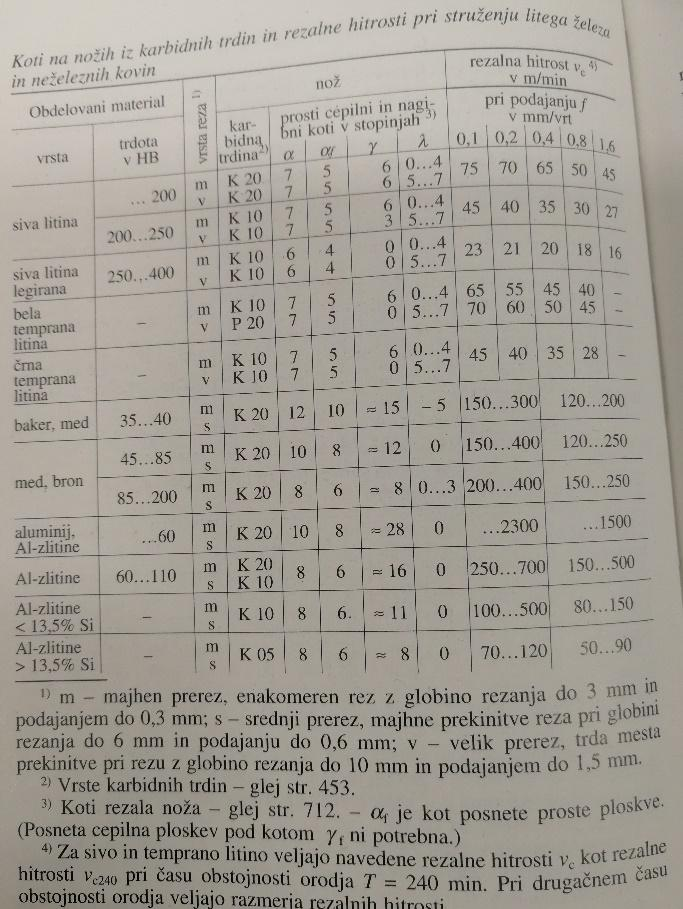
\includegraphics[width=10cm]{rezalne_hitrosti.jpg}
        \caption{Tabela rezalnih hitrosti
        \cite{strojniski_prirocnik}}
        \label{rezalna_hitrost}
    \end{center}
\end{figure}

\newpage
\subsubsection{Vrtanje}
Je operacija obdelave materiala z odrezovanjem. 
Pri vrtanju se lahko vrti orodje ali obdelovanec. Rezultat 
operacije je izvrtina valjaste oblike. Vrtamo z svedri, 
ki imajo za vsak material določen rezni kot in kot vzpona 
vijačnice. Npr. za medenino, je kot vzpona zelo velik, da se 
krhki ostružki hitro odstranijo iz luknje. Za jekla, kjer so 
ostružki največkrat dolgi in nepretrgani, uporabljamo svedre z 
zelo majhnim kotom vzpona.

Svedri za kovino so večinoma narejeni iz hitroreznega jekla in 
prevlečeni z titanovo zlitino.
Naziv »spiralni sveder« ki se ponekod še uporablja je napačen. 
Spirala je krivulja na ravnini, medtem ko je vijačnica krivulja 
skozi prostor, okoli osi.
Poznamo tudi lasersko vrtanje, ki se uveljavlja v zahtevnih 
proizvodnjah, kjer je potrebno izdelati zelo majhne luknje, 
60 - 150 µm, kar z svedri ni mogoče. Lasersko vrtanje pa je zelo 
uporabno tudi pri vrtanju poševnih izvrtin, kar je za običajno 
vrtanje velik izziv.

Za primer imamo spodaj na sliki \ref{hss_sveder} primer navadnega
HSS svedra prevlečenega z titanovo zlitino.
\begin{figure}[H]
    \begin{center}
        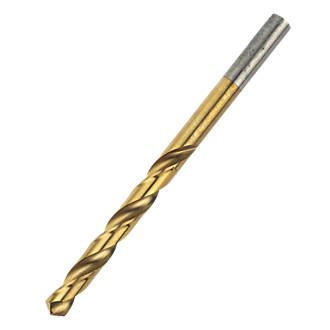
\includegraphics[width=8cm]{sveder.jpg}
        \caption{Navaden HSS sveder
        \cite{sveder}}
        \label{hss_sveder}
    \end{center}
\end{figure}

\newpage
\subsubsection{Povrtavanje}
Je operacija vrtanja, katere namen je izboljšanje točnosti in 
hrapavosti površine v že narejeni izvrtini. Največkrat se 
uporablja ko imamo ujem in moramo doseči gladko površino v 
mejah natančnosti IT6 do IT11. Orodja za povrtavanje, povrtala, 
imajo 6 ali več rezil. Na spodnji sliki \ref{povrtalo} lahko vidimo
primer ročnega povrtala z šestimi rezili.

\begin{figure}[H]
    \begin{center}
        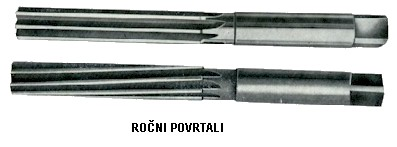
\includegraphics[width=\linewidth]{povrtalo.jpg}
        \caption{Povrtalo
        \cite{sts_arhiv}}
        \label{povrtalo}
    \end{center}
\end{figure}

\subsubsection{Vrezovanje navoja}
Posebna oblika povrtavanja je vrezovanje navoja. Ta operacija se 
lahko izvede samo takrat, ko imamo že predvrtano pravilno 
velikost luknje za dani navoj. Orodja za vrezovanje navojev se 
imenujejo navojni vrezniki, prikazani na spodnji sliki \ref{navojni_sveder}.

\begin{figure}[H]
    \begin{center}
        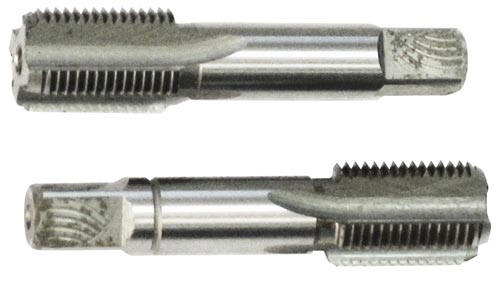
\includegraphics[width=8cm]{navojni.jpg}
        \caption{Navojni sveder
        \cite{sts_arhiv}}
        \label{navojni_sveder}
    \end{center}
\end{figure}

\subsubsection{Grezenje}
Je postopek širjenja že obstoječe. Orodja imenujemo grezila, 
ki vrtajo kvalitetnejšo luknjo kot sveder ali pa pripravlja 
luknjo za povrtavanje. Z grezili dosegamo natančnosti luknje od 
IT8 do IT10. Poznamo tri vrste grezenja: Grobo, fino in oblikovno grezenje.

Za grobo grezenje se največkrat uporablja samo navadni vijačni 
sveder, za fino grezenje uporabljmao grezila, za oblikovno grezenje
pa uporabljamo razna stožčasta enorezilna ali večrezilna grezila 
za oblikovanje izvrtin.
 
Spodaj na sliki \ref{grezilo} je prikazan primer grezenja 
luknje za vijak z konusno glavo.

\begin{figure}[H]
    \begin{center}
        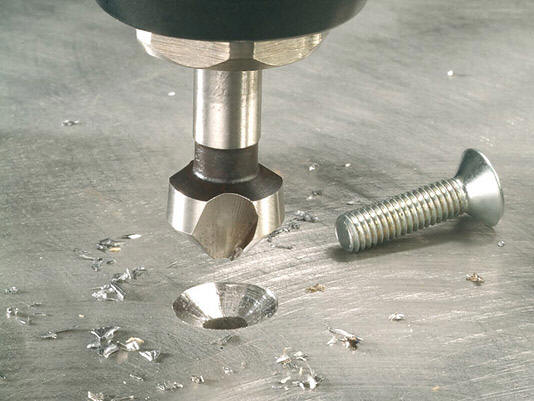
\includegraphics[width=6cm]{grezenje.jpg}
        \caption{Primer grezenja luknje za skritje vijaka
        \cite{sts_arhiv_grezenje}}
        \label{grezilo}
    \end{center}
\end{figure}

\newpage

\subsubsection{Struženje}
Struženje je najbolj razširjen postopek odrezavanja za \
obdelavo valjastih obdelovancev, možno pa je stružiti tudi ravne ploskve 
in celo nekatere neokrogle oblike, če orodje med delom niha.

Glavno gibanje pri struženju je rotacijsko in ga opravlja 
obdelovanec. Podajalno gibanje je navadno premočrtno ali pa 
sledi poljubni krivulji. Struženje zavzema cca. 40\% celotne 
obdelave z odrezavanjem, zato je verjetno struženje najnatančneje
raziskan postopek. Raziskovanja pri struženju so dala vrsto 
zakonitosti, ki so osnove za vse postopke za odrezavanje kovin. 

Poznamo vzdolžno - slika \ref{vzdolzno_struzenje}, 
prečno - slika \ref{precno_struzenje}, stožčasto, profilno,
zarezno struženje - slika \ref{struzenje_utora}, kot tudi struženje navoja, podstruževanje in kopirno struženje.

\begin{multicols}{3}
    \begin{figure}[H]
        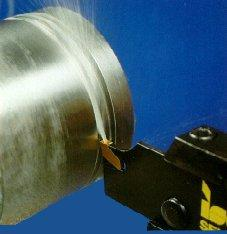
\includegraphics[width=\linewidth]{struzenje_utora.jpg}
        \caption{Struženje utora
        \cite{sts_arhiv_struzenje}}
        \label{struzenje_utora}
    \end{figure}

    \columnbreak

    \begin{figure}[H]
        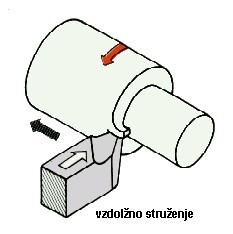
\includegraphics[width=\linewidth]{vzdolzno_struzenje.jpg}
        \caption{Vzdolžno struženje
        \cite{sts_arhiv_struzenje}}
        \label{vzdolzno_struzenje}
    \end{figure}

    \columnbreak

    \begin{figure}[H]
        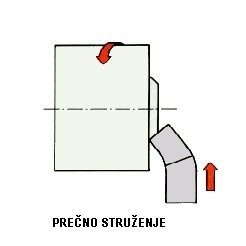
\includegraphics[width=\linewidth]{precno_struzenje.jpg}
        \caption{Prečno struženje
        \cite{sts_arhiv_struzenje}}
        \label{precno_struzenje}
    \end{figure}
\end{multicols}

\newpage
